\documentclass[a4paper]{article}

\usepackage[english]{babel}
\usepackage[utf8]{inputenc}
\usepackage{amsmath}
\usepackage{graphicx}
\usepackage[colorinlistoftodos]{todonotes}

\title{CS5011 Machine Learning Contest Report}

\author{Rishiraj Surti, EE12B120\\
	author2\\
	author3\\}

\date{\today}

\begin{document}
\maketitle

\section{Artificial Neural Network and Sklearn SVM}

\subsection{Artificial Neural Network}

Neural networks are a family of models and are used to estimate and approximate functions that can depend on a large number of inputs. These are inspired by real life Neural networks inside the brain, hence the name.

Neural network (ANN) basically has an input layer, a hidden layer and an output layer. There would be a nonlinear function after every layer to capture the given function.

In this case as the input data is very large we have used large number of hidden neurons so that the model captures the data correctly. Given that the problem is a 100 class classification problem. We have 100 output nodes. Bias is also added to settle the output to the optimum value. We minimized the squared error loss in the process of training. The learning rate is kept low so that the function settles to a good optimum value.

\subsection{Sklearn SVM}

Support Vector Machines are supervised learning models with associated learning algorithms that analyse and recognize patterns used for classification and regression.

SVM's come under the class of "directly modelling a separating hyperplane".
There are many hyperplanes that might classify the data. One reasonable choice as the best hyperplane is the one that represents the largest separation, or margin, between the two classes. So we choose the hyperplane so that the distance from it to the nearest data point on each side is maximized. If there exists no hyperplane that can split the "yes" and "no" examples, the Soft Margin method will choose a hyperplane that splits the examples as cleanly as possible, while still maximizing the distance to the nearest cleanly split examples.

We have used RBF kernel, Sigmoid kernel and the results were not satisfactory.

\section{LDA, QDA, KNN}

\section{LibSVM, Bayes, Adaboost}
\subsection{LibSVM}

\begin{table}
\centering
\begin{tabular}{l|l|l}
Algorithm & Source File & Output file \\\hline
SVM & svm\_rs.py & svm\_rs\_output\_*.py \\

\end{tabular}
\caption{\label{tab:widgets}List of files}
\end{table}




\begin{figure}
\centering
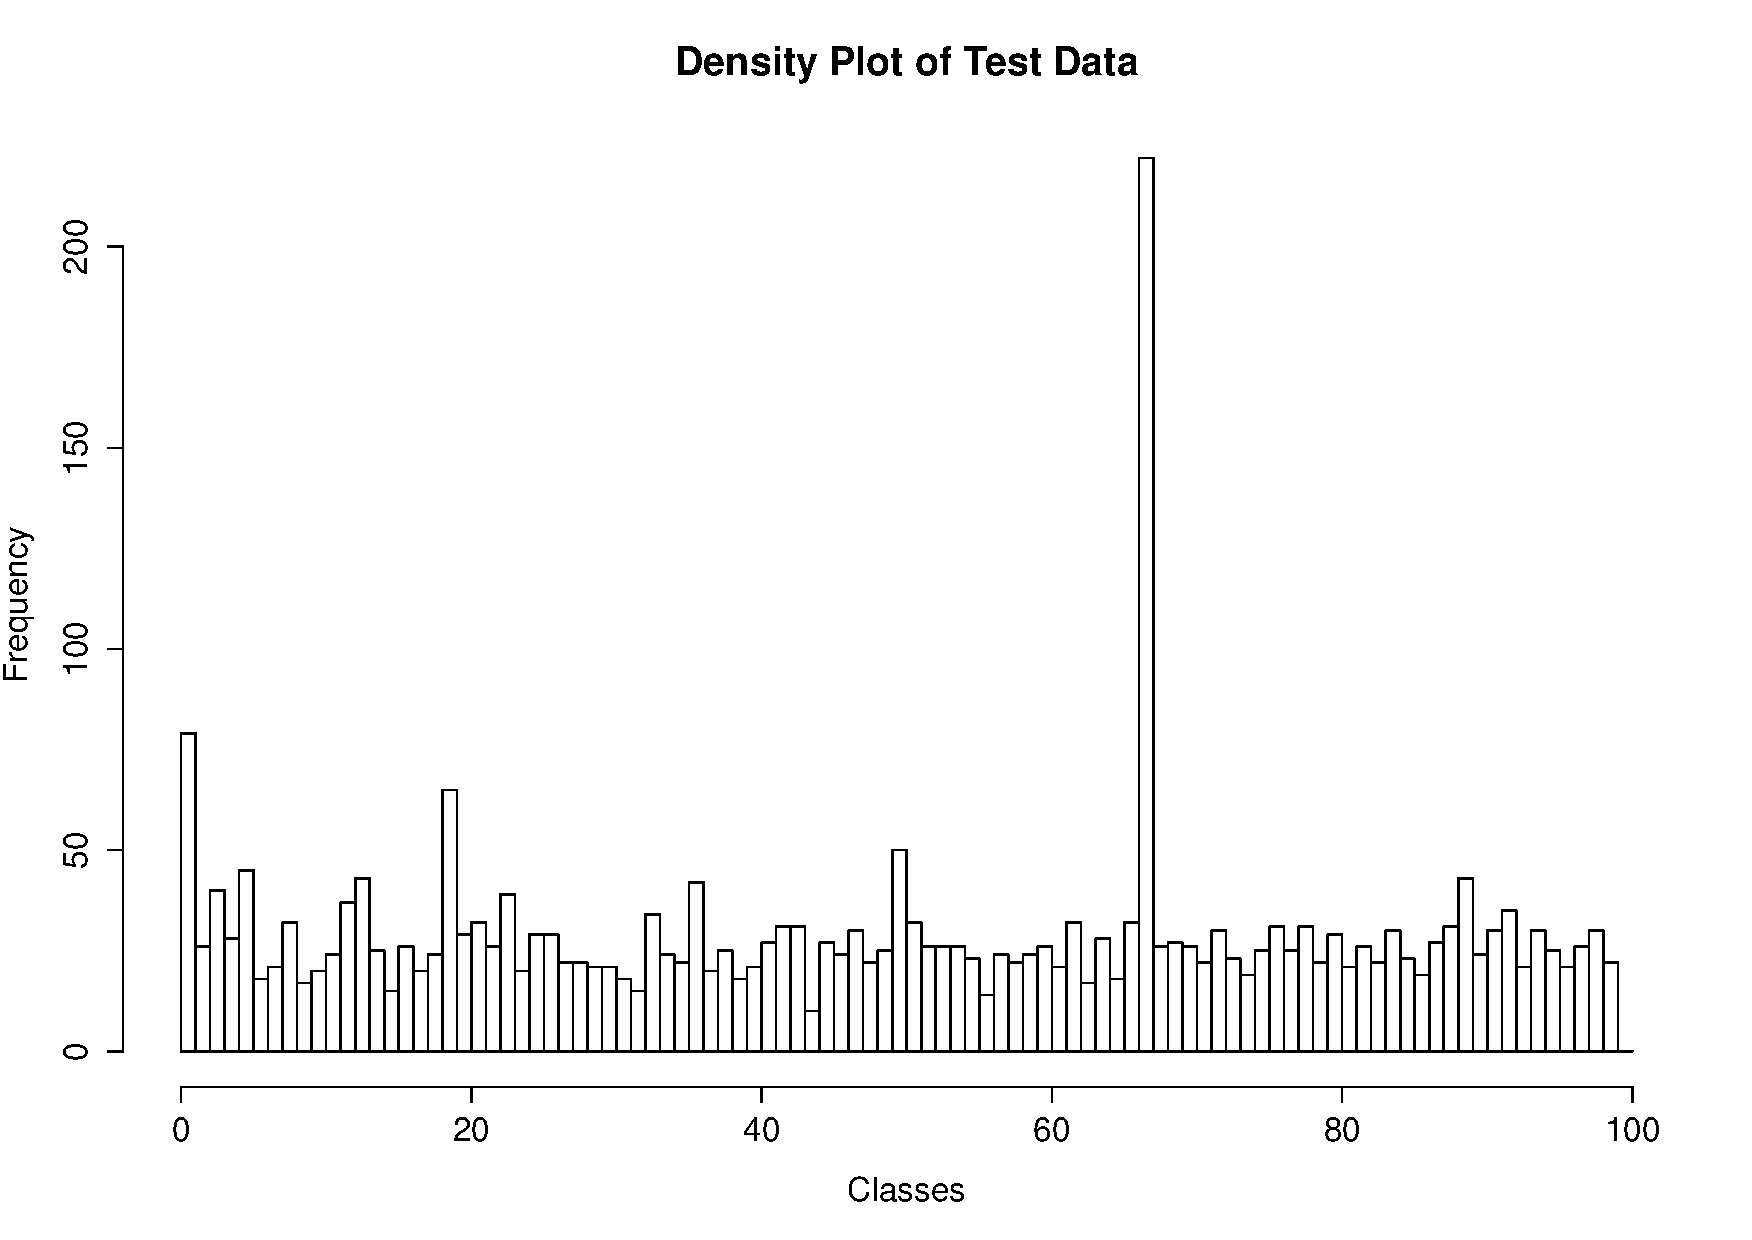
\includegraphics[width=1\textwidth]{../plots/TestData_targets.pdf}
\caption{\label{fig:data}Raw (unprocessed) data. Replace this figure with the one you've made, that shows the resistivity.}
\end{figure}

\begin{table}
\centering
\begin{tabular}{l|r}
Item & Quantity \\\hline
Widgets & 42 \\
Gadgets & 13
\end{tabular}
\caption{\label{tab:widgets}An example table.}
\end{table}


\begin{enumerate}
\item Like this,
\item and like this.
\end{enumerate}
\dots or bullet points \dots
\begin{itemize}
\item Like this,
\item and like this.
\end{itemize}
\dots or with words and descriptions \dots
\begin{description}
\item[Word] Definition
\item[Concept] Explanation
\item[Idea] Text
\end{description}

\end{document}
              
